% 
% Annual Cognitive Science Conference
% Sample LaTeX Paper -- Proceedings Format
% 

% Original : Ashwin Ram (ashwin@cc.gatech.edu)       04/01/1994
% Modified : Johanna Moore (jmoore@cs.pitt.edu)      03/17/1995
% Modified : David Noelle (noelle@ucsd.edu)          03/15/1996
% Modified : Pat Langley (langley@cs.stanford.edu)   01/26/1997
% Latex2e corrections by Ramin Charles Nakisa        01/28/1997 
% Modified : Tina Eliassi-Rad (eliassi@cs.wisc.edu)  01/31/1998
% Modified : Trisha Yannuzzi (trisha@ircs.upenn.edu) 12/28/1999 (in process)
% Modified : Mary Ellen Foster (M.E.Foster@ed.ac.uk) 12/11/2000
% Modified : Ken Forbus                              01/23/2004
% Modified : Eli M. Silk (esilk@pitt.edu)            05/24/2005
% Modified : Niels Taatgen (taatgen@cmu.edu)         10/24/2006
% Modified : David Noelle (dnoelle@ucmerced.edu)     11/19/2014

%% Change "letterpaper" in the following line to "a4paper" if you must.

\documentclass[10pt,letterpaper]{article}

\usepackage{cogsci}
\usepackage{pslatex}
\usepackage{apacite}
\usepackage{graphicx}
\usepackage{color}


\definecolor{Red}{RGB}{255,0,0}
\newcommand{\red}[1]{\textcolor{Red}{#1}}

\newcommand{\subsubsubsection}[1]{{\em #1}}
\newcommand{\eref}[1]{(\ref{#1})}
\newcommand{\tableref}[1]{Table \ref{#1}}
\newcommand{\figref}[1]{Figure \ref{#1}}
\newcommand{\appref}[1]{Appendix \ref{#1}}
\newcommand{\sectionref}[1]{Section \ref{#1}}

\title{Non-sinking marbles are wonky: defeasible world knowledge in language interpretation}
 
\author{{\large \bf Judith Degen (jdegen@stanford.edu)} %\\
  \AND {\large \bf Michael H.~Tessler (mtessler@stanford.edu)} \\
  \AND {\large \bf Noah D.~Goodman (ngoodman@stanford.edu)} \\
  Department of Psychology, 450 Serra Mall \\
  Stanford, CA 94305 USA}

% ggplot colors: "#F8766D", "#A3A500", "#00BF7D", "#E76BF3", "#00B0F6"

\begin{document}

\maketitle


\begin{abstract}
World knowledge enters pragmatic utterance interpretation in complex ways. Sometimes, a speaker's utterance suggests that listeners should disregard their world knowledge, yet current models of pragmatic interpretation either disregard the role of world knowledge or overestimate its role in interpretation. Here we provide an extension to the Rational Speech Act model of scalar implicature that captures whether listeners believe they are in an abnormal--or `wonky'--world after observing a speaker's utterance, in which case they downweight their prior beliefs in the computation of speaker meaning. We show in four experiments that a) listeners have varying prior beliefs about the probability of various objects exhibiting an effect (e.g., marbles sinking), b) these beliefs influence listeners' expectations about how many objects will show the effect after observing an utterance (like \emph{Some of the marbles sank}), c) these beliefs influence scalar implicature strength, and d) listeners' world wonkiness judgments are affected by the surprisal of the observed utterance under their prior beliefs. The extended model is the first quantitative model that accounts for how rational listeners should integrate world knowledge in pragmatic utterance interpretation, and provides a close match to the empirically obtained data.

\textbf{Keywords:} 
scalar implicature; world knowledge; prior beliefs; experimental pragmatics; computational pragmatics
\end{abstract}

How often do you think marbles would sink in water? Probably quite often, if not always. Now imagine reading \emph{Max threw his favorite marbles in the water. Some of them sank.} Have you begun to reconsider your assumptions? Perhaps you now suspect that these marbles are in fact made of plastic or the water is enriched with something that makes them float? That is, that they are not just normal marbles in normal water. Here we explore how prior world knowledge enters into pragmatic utterance interpretation, and how this world knowledge is defeasible: some utterances lead listeners to conclude that the world under discussion is abnormal under their prior beliefs, or, to use the technical term, the world is \emph{wonky}.


%World knowledge enters into the interpretation of utterances in complex ways. %For example, the plausibility of an NP as the subject of a sentence influences whether listeners are garden-pathed in cases like \textit{The horse raced past the barn fell} vs.~\textit{The landline buried in the sand exploded} \cite{bla}.
%While effects of world knowledge on syntactic processing are well-established, there is to date a surprising lack of systematic investigations into the effect of world knowledge in pragmatics. % -- this is especially surprising given that it has long been noted in the linguistics literature that pragmatics requires the integration of many different sources of linguistic and non-linguistic information. 
%Here, we provide a quantitative model of the effect of world knowledge  on  scalar implicatures, which are inferences that arise in cases of utterances like \textit{Some of the marbles sank}, %like (\ref{marbles}), where an utterance of (\ref{somemarbles}) 
%which typically gives rise to the inference that not all of the marbles sank.% in (\ref{simarbles}).
%
%\begin{exe}
%	\ex\label{marbles} 
%	\begin{xlist}
%		\ex\label{somemarbles} Some of the marbles sank.
%		\ex\label{simarbles} Not all of the marbles sank.
%	\end{xlist}
%\end{exe}

\section{Models of utterance interpretation}

Recent Bayesian Rational Speech Act (RSA)  \cite{frank2012} and game-theoretic \cite{franke2011} models treat communication as a signaling game \cite{lewis} between a speaker and a listener, in which a listener iteratively reasons about likely utterances a speaker will produce who is trying to be informative with respect to a na\"ive listener. These models make clear predictions about how prior beliefs about states $s$ of the world should be integrated with listeners' expectations about utterances $u$ a speaker is likely to produce to communicate $s$. 

%For concreteness, assume that $S = \{s_0, s_1, s_2, \dots, s_{15}\}$ is the set of states of the world, where the subscript indicates the number of objects (e.g., marbles) that exhibit a certain effect (e.g., sinking). Assume further that $U = \{u_{\textrm{all}}, u_{\textrm{none}}, u_{\textrm{some}}, u_{\textrm{null}}\}$, corresponding to the sentences \emph{all/none/some of the marbles sank} and $u_{\textrm{null}}$ corresponding to a cheap alternative utterance (e.g., silence) that does not communicate any new information about the world.

\red{INTRODUCE SPEAKER UTILITY RULE AT SOME POINT IN THIS PARAGRAPH} The listener's task can be characterized as having to infer $p(s|u)$, that is, the probability of the state of the world the speaker intended to communicate (e.g., how many friends came to a party), given that the speaker produced $u$ (e.g., \emph{some of my friends came to the party}). By Bayes' rule: $p(s|u)\propto p(u|s)\cdot p(s)$. That is, the inferred listener probabilities are proportional to the product of the speaker's utterance probabilities and the listener's prior beliefs in different numbers of friends coming to the party. As a consequence, the listener's prior beliefs will not affect the interpretation of $u$ very strongly, if at all,  where the semantics of  $u$ is highly constraining with respect to $s$. For example, an utterance of \emph{all of my friends came to the party} will constrain the state space to include only the state in which all of the friends came, regardless of how likely the listener believes the speaker's friends are to show up a priori.\footnote{We ignore hyperbolic interpretations of universal quantifiers here.} In contrast, where the semantics of $u$ is weak -- that is, if $u$ does not constrain the state space the listener is considering very strongly -- prior beliefs are predicted to have a large effect on the resulting listener belief distribution over $s$. For example, an utterance of \emph{some of my friends came to the party}, produced in a situation in which any of 0 - 15 of 15 contextually established friends could have come, semantically only restricts the state space by one state (that in which 0 friends came). In this case, listeners' prior beliefs about the speaker's friends coming will have a large effect on their posterior belief distribution. If the speaker's friends rarely show up, her utterance will be interpreted as conveying that fewer of her friends came than if they almost always show up.

However, as evident in the introductory sinking marbles example, prior beliefs about the world are defeasible. \red{EXPAND AND INTRODUCE THE INTUITION ABOUT THE SPEAKER'S UTTERANCE TRIGGERING DEFEASIBILITY} The currently available models of utterance interpretation either do not take into account world knowledge in the form of prior beliefs at all \red{some refs} or do not allow for their defeasibility \red{RSA/game-theoretic refs}.

Here we measure the effect of world knowledge and its defeasibility in the interpretation of utterances that contain quantifiers like \emph{all/none/some of the marbles sank}. While the semantics of \emph{all} and \emph{none} are highly constraining and limit the state space to just one state (that in which either zero or all of the marbles sank, respectively), the semantics of \emph{some} is weak and is compatible with many different states of the world, as long as more than zero marbles sank. In addition, utterances with \emph{some} give rise to scalar implicatures \cite{grice1975}. These are inferences that arise in cases of utterances like \textit{Some of the marbles sank}, which typically give rise to the inference that not all of the marbles sank (or else the speaker would have said so). 

We refer to the state in which all marbles sink as $s_{\forall}$ and the utterance with \emph{some} as $u_{\textrm{some}}$. Without further modification, RSA predicts that $p(s_{\forall}|u_{\textrm{some}})$ increases with increasing $p(s_{\forall})$, such that for $p(s_{\forall})$ close to 1, $p(s_{\forall}|u_{\textrm{some}})$ approaches 1, that is, implicatures are very weak (see Figure \red{XXX create}). Relatedly, with increasing expected value of the prior belief distribution, so is the expected value of the posterior belief distribution predicted to increase (see \figref{fig:rrsaexppredictions}).   However, intuition is at odds with this prediction: for events with very high prior probability of occurrence (e.g.~marbles sinking), the implicature that not all of the marbles sank is intuitively very strong, that is, $p(s_{\forall}|u_{\textrm{some}})$ should be close to 0 \cite{geurts2010}. \red{Given the previous success of RSA models, this constitutes a striking puzzle, and one we set out to solve here.}

Our contribution is two-fold: first, we collect empirical estimates of $p(s)$ and $p(s|u)$ to investigate the empirical effect of listeners' prior beliefs on implicature strength. Second, we extend the RSA model to incorporate a free variable $\theta_{\textrm{wonky}}$ that captures the extent to which the listener believes the described event is abnormal or `wonky'  and she should thus discount her prior beliefs when interpreting $u$. We refer to this model as \textit{wonky RSA} (wRSA) in contrast to \textit{regular RSA} (rRSA). Wonkiness inferences in wRSA are triggered by the surprisal of a produced utterance $u$, given listeners' prior beliefs, capturing that listeners expect speakers' utterances to be both truthful and informative with respect to prior beliefs. To the extent that they are not, listeners will have to either infer that the speaker is being uncooperative, or else assume that they may need to revise their beliefs about the world. Here we pursue the latter possibility.

This paper is structured as follows. We first report the results of three experiments (1, 2a, 2b) that show that while there is an effect of the prior on listeners' interpretations of sentences like \emph{Some of the marbles sank}, this effect is much smaller than predicted by rRSA. Exp.~3 provides evidence that listeners' beliefs about object or event wonkiness are indeed influenced by the surprisal of the utterance. Finally, we present an extension of rRSA that incorporates the idea of backing off to alternate prior beliefs if the observed utterance indicates a wonky world. This model provides a much better fit to the empirical data from Exps.~2a and 2b, and also provides a good fit to the wonkiness ratings obtained in Exp.~3.

\begin{figure}
	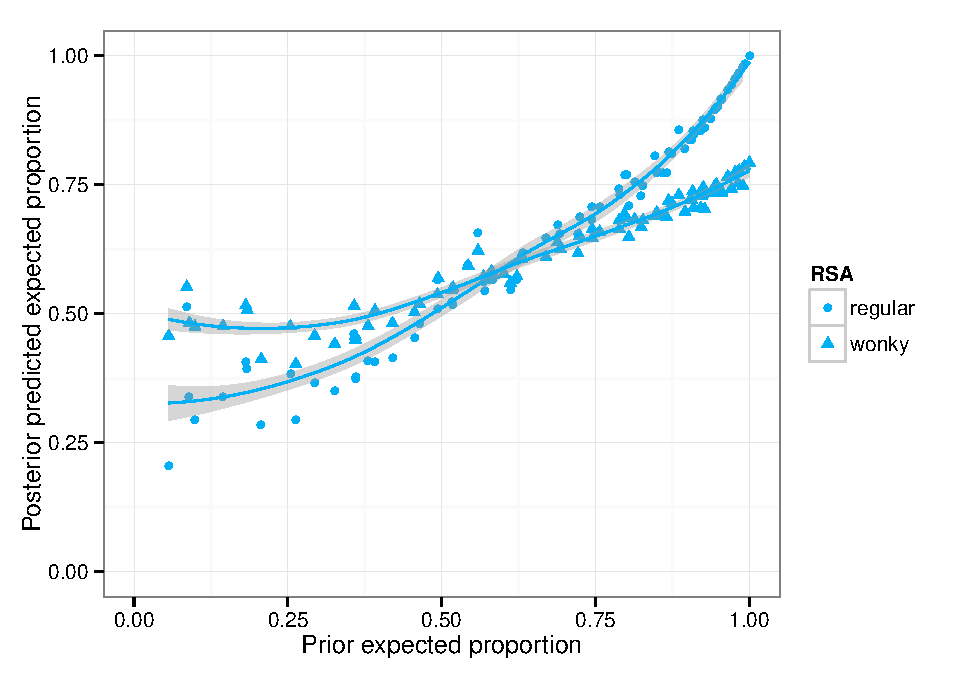
\includegraphics[width=.5\textwidth]{pics/model-expectations-uniform-regular}
	\caption{For each item, rRSA and wRSA model predicted mean empirical proportion of affected objects after observing \emph{Some of the X Yed}, as a function of prior mean proportion of affected objects.}
	\label{fig:rrsaexppredictions}	
\end{figure}

\red{Include also plot of all-state probability: posterior empirical and predicted probability (rRSA, wRSA) as a function of prior all-state probability, for the SI people}

\section{Experiment 1} 

Exp.~1 measured $p(s)$, participants' prior beliefs about different objects exhibiting a certain effect (e.g., marbles sinking).

\subsection{Method}

\subsubsection{Participants}
We recruited 60 participants over Amazon�s crowd-sourcing platform Mechanical Turk.

\subsubsection{Procedure and materials}

On each trial, participants read a description of an event like \textit{John threw 15 marbles into a pool.} They were then asked to provide a judgment of an effect, e.g.~\textit{How many of the marbles do you think sank?}, on a sliding scale from 0 to 15. Judgments were obtained for 90 items, of which each participant saw a random selection of 30 items.

\subsection{Results}

Data from one participant, who gave only one response throughout the experiment, were excluded. Each item received between 12 and 29 ratings. Distributions of ratings for each item were smoothed using nonparametric density estimation for ordinal categorical variables \cite{liracine2003} using the \verb|np| package in R \cite{hayfield2013} \red{see hayfield 2013 np package specification for li and racine ref}.

\section{Experiment 2a}  

Exp.~2a measured $p(s|u)$,   participants' posterior beliefs in different objects exhibiting a certain effect (e.g., marbles sinking), after observing an utterance. 

\subsubsection{Participants}
We recruited 120 participants over Amazon�s crowd-sourcing platform Mechanical Turk.

\subsubsection{Procedure and materials}

Participants read the same descriptions as in Exp.~1. They additionally saw an utterance produced by a knowledgeable speaker about the event, e.g.~\textit{John, who observed what happened, said: ``Some of the marbles sank''}, and were asked to rate on sliding scales with endpoints labeled ``very unlikely'' and ``very likely'', how likely they thought 0\%, 1-50\%, 51-99\%, or 100\% of the marbles sank.


 Each participant saw 10 ``some'' trials and 20 fillers, of which 10 contained the quantifiers ``all'' or ``none'', and the rest were utterances that did not address the number of objects that displayed the effect, e.g.~\textit{What a stupid thing to do.} 
 
 \subsubsection{Results}
 \red{XXX question}

 $p(s_{\forall}|u_{\textrm{some}})$ increased with increasing \red{talk about both $p(s_{\forall}$ and the prior expectation of the distribution?} $p(s_{\forall}$) ($\beta$=.1, $SE$=.01, $t$=6.9, $p$$<$.0001); however, mean $p(s_{\forall}|u_{\textrm{some}})$ was never higher than .26, suggesting that a) participants drew strong implicatures in this paradigm and b) the effect of $p(s)$ is much smaller than predicted by rRSA.

\section{Experiment 2b}  

Exp.~2b replicates the effect of the prior on participants' posterior estimates of different objects exhibiting a certain effect (e.g., marbles sinking) using a different dependent measure. 

\subsubsection{Participants}
We recruited 120 participants over Amazon�s crowd-sourcing platform Mechanical Turk.

\subsubsection{Procedure and materials}

The procedure and materials were identical to those of Exp.~2a with the exception of the dependent measure. Rather than providing point estimates of the probability of different numbers of objects sinking, participants performed the task from Exp.~1, i.e., they were asked to provide a judgment of an effect, e.g.~\textit{How many of the marbles do you think sank?}, on a sliding scale from 0 to 15.
 
 \subsubsection{Results and discussion}
 \red{XXX question}

The mean number of objects judged to exhibit the effect increased with increasing expectation of the prior distribution ($\beta$=.18, $SE$=.02, $t$=7.4, $p$$<$.0001, see also \figref{fig:meanresponses}), replicating the effect observed in Exp.~2a. Again, the effect of the prior was much smaller than predicted by rRSA and resulted in mean proportions of affected objects between 30\% and 65\%, where rRSA predicts a range from \red{XXX} to \red{XXX} for these items.


\begin{figure}
	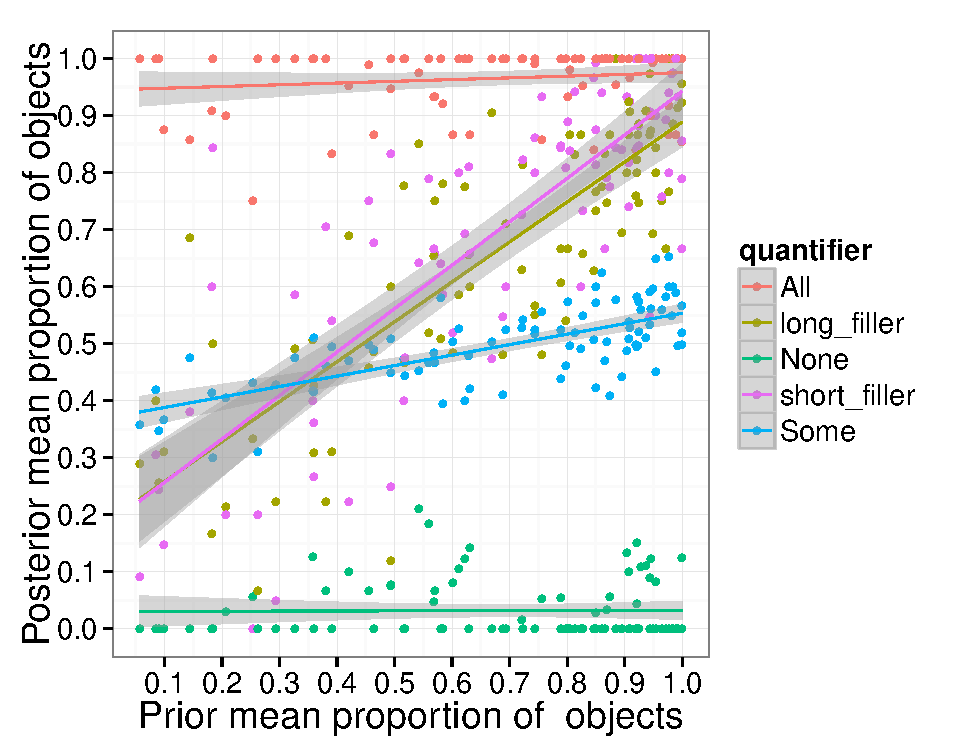
\includegraphics[width=.5\textwidth]{pics/meanresponses}
	\caption{For each item, mean empirical proportion of affected objects after observing an utterance, as a function of prior mean proportion, for different quantifiers and filler conditions.}
	\label{fig:meanresponses}	
\end{figure}

Exps.~2a and 2b demonstrate that there is a robust effect of listeners' prior beliefs on the interpretation of utterances with \emph{some}. However, this effect is much smaller than predicted by rRSA. 

\red{Discussion of why; wonky world intuition}

\section{Experiment 3}

Exp.~3 measured participants' beliefs in world wonkiness after observing the scenarios and utterances from Exps.~2a and 2b.

\subsubsection{Participants}
We recruited 60 participants over Amazon�s crowd-sourcing platform Mechanical Turk.

\subsubsection{Procedure and materials}

The procedure and materials were identical to those of Exps.~2a and 2b, with the exception of the dependent measure. Rather than providing estimates of what they believed the world was like, participants were asked to indicate whether they believed the objects  (e.g., the marbles) involved in the scenario were normal objects, by clicking a `Yes' or `No' radio button.

\subsubsection{Results}

Proportion of `No' ratings (where we take `No' ratings to indicate participants belief in wonkiness of the world) for each item and quantifier are shown in \figref{fig:wonkyratings}. For `all' and `none', increasing prior expectation of objects exhibiting the effect results in a monotonic decrease and increase in the probability of wonkiness, respectively. For `some', the pattern is somewhat more intricate: probability of wonkiness initially decreases sharply, but rises again in the upper prior expectation range. 

\begin{figure}
	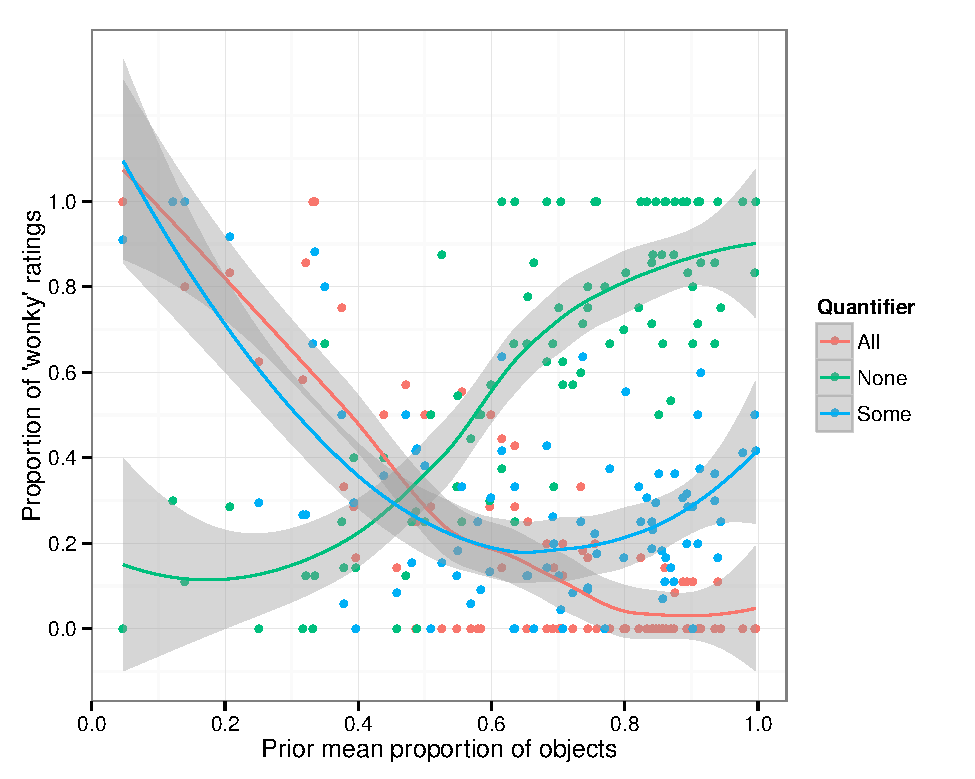
\includegraphics[width=.5\textwidth]{pics/proportionwonky-empirical}
	\caption{For each item, empirical proportion of 'wonky' ratings after observing an utterance, as a function of prior mean proportion, for different quantifiers.}
	\label{fig:wonkyratings}	
\end{figure}

\red{yay!! XXX}

\section{Model}

\red{continue exploring priors before reporting}

\red{From the CUNY abstarct: In wRSA, the listener infers the value of $\theta_{\textrm{wonky}}$ jointly with $s$. $\theta_{\textrm{wonky}}$ captures for each utterance and item, how likely the objects involved in the event (e.g., marbles) are in fact ``wonky'' (in which case the computation draws on a uniform prior, i.e.~disregards prior beliefs) or not (in which case the model draws on the smoothed empirical prior distribution for that item, obtained in Exp.~1). The resulting $p(s|u)$ is a mixture of computations based on the uniform and empirical prior, with mixture parameter $\theta_{\textrm{wonky}}$. The inferred value of $\theta_{\textrm{wonky}}$ itself depends on $p(u|s)$: the more surprising a particular utterance is given prior beliefs, the higher the probability of $\theta_{\textrm{wonky}}$.}


\section{Model evaluation}

\begin{figure}

	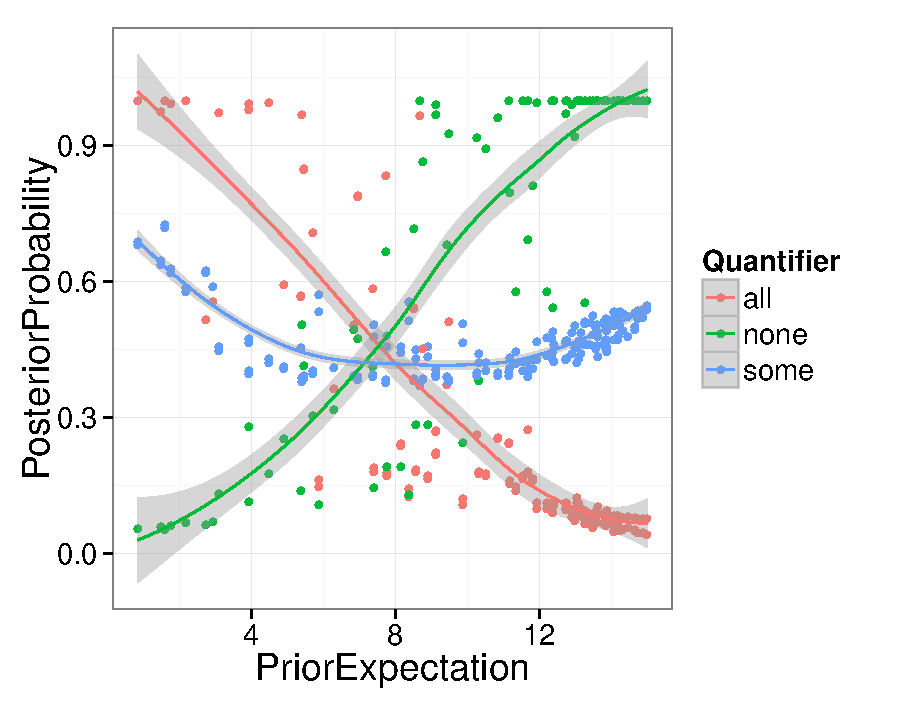
\includegraphics[width=.5\textwidth]{pics/proportionwonky-model}
	\caption{\red{For each item, predicted proportion of 'wonky' ratings after observing an utterance, as a function of prior mean proportion, for different quantifiers.}}
	\label{fig:wonkymodel}	
\end{figure}

\red{From the abstract: Comparing the fit of rRSA and wRSA model predictions to the posterior state estimates from Exp.~2 yields a much better fit for wRSA. The better fit of wRSA suggests that listeners  use speakers' utterances as cues to how strongly to incorporate world knowledge. wRSA also provided a better fit than a model which used only a uniform prior, confirming that listeners do make use of world knowledge in a systematic way in the computation of scalar implicature.}





\section{General discussion}

\begin{itemize}

	\item what is wonky?
	\item other ways of asking about wonkiness
	\item what's the right prior to back off to?

\end{itemize}

\section{Conclusion}


\bibliographystyle{apacite}

\setlength{\bibleftmargin}{.125in}
\setlength{\bibindent}{-\bibleftmargin}

\bibliography{bibs}


\end{document}
